\chapter{Обзор литературы}\label{ch:ch1}
\nomenclature{ОДУ}{Обыкновенное дифференциальное уравнение}
\nomenclature{ДАУ}{Дифференциальное алгебраическое уравнение}
\nomenclature{ВАК}{Высшая аттестационная комиссия}
\section{Шагающие роботы}\label{sec:ch1/sec1}

Шагающие роботы предлагают больше возможностей по сравнению с колёсными и гусеничными роботами с точки зрения условий работы. Шагающие роботы могут передвигаться по обычной и неровной местности без каких-либо аппаратных изменений и демонстрируют исключительную мобильность \cite{Silva2012}. Колёсные транспортные средства требуют для передвижения асфальтированных (или хотя бы сглаженных) поверхностей, но при этом они чрезвычайно быстры и эффективны на них. Также колёсные механизмы в большинстве случаев являются лёгкими и простыми в конструировании и использовании \cite{Zen2006}. Однако более 50 процентов поверхности Земли недоступно для традиционных транспортных средств, и колёсным машинам трудно или даже невозможно справиться с большими препятствиями и неровностями поверхности. Вездеходы могут преодолевать лишь небольшие препятствия и неровности, но только за счёт высокого потребления энергии \cite{Bekker1962}. Что касается гусеничных машин, то, хотя они и обеспечивают повышенную мобильность на сложных участках, они не в состоянии преодолеть многие препятствия, а их энергопотребление относительно велико. К этим проблемам следует добавить тот факт, что традиционные транспортные средства оставляют на земле сплошные колеи, что в некоторых ситуациях неприменимо, например, с экологической точки зрения. 

Из всего вышесказанного можно сделать вывод, что системы передвижения на ногах обеспечивают лучшую мобильность на естественных участках местности, поскольку эти транспортные средства могут использовать отдельные опоры для каждой ноги, в отличие от колёсных транспортных средств, которым необходима непрерывная опорная поверхность. Шагающие роботы могут передвигаться по неровной местности, изменяя конфигурацию ног, чтобы адаптироваться к неровностям поверхности, и, кроме того, ноги могут устанавливать контакт с землёй в отдельных точках в соответствии с условиями местности. Когда транспортные средства передвигаются по мягким поверхностям, например, по песчаной почве, возможность использовать дискретные опоры в грунте может также улучшить энергопотребление, поскольку они деформируют рельеф меньше, чем колёсные или гусеничные транспортные средства \cite{Iida2007}. 

Энергия, необходимая для выхода из углублений шагающему роботу, меньше \cite{Bekker1962, bekker1969}, а площадь контакта стопы с землёй может быть такой, чтобы давление на опору было небольшим. Кроме того, использование нескольких степеней свободы в суставах ног позволяет шагающим роботам менять направление движения без проскальзывания. Также можно варьировать высоту корпуса, создавая эффект демпфирования и развязки между неровностями рельефа и кузовом транспортного средства (и, как следствие, его полезной нагрузкой). Что касается движения, то следует также упомянуть о возможности, которую предоставляют эти системы, прижиматься к местности, по которой они движутся. Это особенно верно, если они перемещаются, например, по внешней поверхности труб, чтобы повысить способность к балансировке \cite{Kaneko2002}.

Четвероногие роботы --- лучший выбор среди всех ножных роботов с точки зрения мобильности и стабильности управления. Четыре ноги робота легко контролируются, проектируются и обслуживаются по сравнению с двумя или шестью ногами. Биологически вдохновлённая локомоция беговой походки способна выдержать большую полезную нагрузку и балансировку четвероногого робота. Для достижения скорости в реальном времени и естественного движения, как у коровы, собаки, гепарда, необходима разработанная система управления и динамическая генерация походки четвероногих роботов \cite{gonccalves2013}.

Четырёхногие роботы вдохновлены локомоцией четвероногих животных: шарнирные соединения в коленях, бёдрах и шее позволяют им повторять их движения. Самый ранний пример такого робота датируется 1870 годом, когда Чебышев сконструировал четвероногий механизм, который мог стоять и ходить, но не мог адаптироваться к местности \cite{Cheb1948}. В 1893 году Рюгг получил первый патент на ножную машину --- симулятор верховой езды, приводимый в движение педалями \cite{patent}. Заметный шаг в развитии четвероногих роботов произошёл в 1940 году, когда Хатчинсон сконструировал автономно управляемого робота на ногах, подчёркивая преимущества педальных систем перед колёсными или гусеничными машинами для работы с тяжёлыми грузами \cite{Hutchinson1967}.  Кульминацией этого подхода стала постройка компанией \textit{Bucyrus--Eire} в 1969 году самой большой машины на ногах \textit{Big Muskie} \cite{haddock2001extreme}. Этот массивный робот проработал в открытых карьерах 22 года, продемонстрировав целесообразность использования четвероногих механизмов для крупномасштабных промышленных применений.

В 1980-х годах профессор Хиросэ из Токийского технологического института создал семейство четвероногих роботов, ключевой вехой которого стал \textit{PV-II}. Этот робот оснащён моторизованным приводом для каждой ноги, что позволяет ему эффективно ходить \cite{Hirose2009}. Дальнейшие разработки, такие как четвероногий робот \textit{OSQ} из Стэнфорда, продвинули понимание галопирующей походки и энергоэффективного передвижения \cite{Nichol2004}.  Совсем недавно китайские институты, такие как Шаньдунский университет, разработали четвероногих роботов \textit{SCalf--1} и \textit{SCalf--2}, оснащённых усовершенствованными гидравлическими системами для улучшения адаптации к местности и повышения скорости \cite{Rong2012}.

Несмотря на все потенциальные преимущества шагающих роботов, на текущем этапе развития есть несколько аспектов, которые необходимо улучшить и оптимизировать. Одним из недостатков является сложность законов управления. В большинстве случаев, среди всех необходимых вычислений, требуются обратные матрицы инерции жёсткого тела в нескольких местах, что делает этот подход чувствительным к ошибкам моделирования и оценки параметров \cite{Nakanishi_IJRR_2008}. 

\section{Управление для шагающих роботов}\label{sec:ch1/sec2}

Управление подвижными шагающими роботами представляет собой сложную задачу из--за недостаточной динамики тела во время шагов и из--за ограничений, накладываемых на силы реакции на грунт. Исследования в основном были сосредоточены на определении положения и ориентации основания, а также каждой ноги, при рассмотрении системы четвероногих роботов как плавающей в пространстве системы с несколькими телами. Переменные состояния включают в себя конфигурацию тела и углы сочленения ног. Управляющие силы в системе включают крутящие моменты в суставах и силы реакции на грунт.

Желаемая траектория движения тела и каждой ноги может быть сформирована с помощью предварительного планирования или включение ограничений. Помимо ограничений, связанных с контактом с землёй и трением, задачи могут быть описаны в виде уравнений или неравенств, включающих переменные состояния или моменты вращения суставов. Чтобы решить проблему противоречивых ограничений задачи, необходимо использовать соответствующие уравнения оптимизации при проектировании иерархического управления. Такой иерархический регулятор, известный как регулятор всего тела \cite{fahmi2019passive}, объединяет задачи для всех систем робота. 

Планирование и управление движением занимают центральное место в работе четвероногих роботов, включая формирование и выполнение походки. К распространённым методам формирования походки относятся генераторы центрального паттерна, модель перевёрнутого маятника с пружинной нагрузкой, метод нулевой точки момента и траектории кривых Безье.

Модельное прогнозирующее управление --- это метод итеративного решения проблем оптимизации на основе режимов, учитывающий текущее состояние системы и прогнозирующий его изменение в будущем \cite{KIM2019}. Использование управления с прогнозирующими моделями повышает универсальность локомоции, позволяя переключаться между различными походками, просто меняя последовательность контактов. Однако использование управления с прогнозирующими моделями с простой моделью имеет фундаментальное ограничение в управлении положением из--за низкой частоты обновления и упрощения модели. 

В последнее время в научной литературе наблюдается растущий интерес к оптимизационным методам планирования траекторий и управления шагающими роботами. Это связано с высокой эффективностью этих методов, их способностью учитывать различные ограничения, иерархию задач, механические связи и другие факторы. Появление высокопроизводительных вычислителей и эффективных алгоритмов для решения задач выпуклого программирования открыло новые возможности для применения таких методов управления. Существует значительное разнообразие разработанных методов оптимизационного управления, которое не имеет чёткой систематизации. Кроме того, отсутствуют методологии для анализа устойчивости и робастности этих систем управления, а также интегрированные подходы к планированию последовательностей шагов и выбору управляющих воздействий.

Выпуклая оптимизация позволяет обойтись без методов нелинейной оптимизации, которые, в отличие от решателей выпуклой оптимизации, не гарантируют нахождения глобального оптимума и могут страдать от численных проблем \cite{boyd2004convex}. Стабилизация четвероногого робота \textit{HyQ} с помощью выпуклой оптимизации, рассмотренная в \cite{Focchi2016}, демонстрирует практичность выпуклой оптимизации, но этот подход не может быть немедленно распространён на динамические походки из-за  упрощений, внесённых в модель робота.

\section{Ортогональные методы}\label{sec:ch1/sec3}

Существует целый ряд работ по проектированию управления для очень большого класса систем, описываемых ДАУ или вырожденными ОДУ, называемых дескрипторными системами. В этой области исследований есть результаты по робастному управлению и проектированию наблюдателей \cite{Cheng2018, Darouach2014}. Однако методы, разработанные в этой области, недостаточны для решения проблемы, рассматриваемой в данном диссертационном исследовании. В работе \cite{Aghili2003} была предложена процедура для моделирования механических систем с явными ограничениями, что устанавливает связь с более ранними работами в области численных методов для ДАУ, такими как \cite{Liang1987} и другие, в которых рассматривалась очень похожая проблема. 

Для дескрипторных систем с неопределённостями были разработаны методы построения законов управления, например в работах \cite{Darouach2014, LIN19993319}. Однако, при работе с ДАУ и введением в систему неопределённостей возникает необходимость допущений, например, введение условия на структуру и ранг дифференциальной матрицы \cite{Cheng2017}, увеличение сложности точных вычислений для больших размерностей \cite{Zhang2006}. 

Численные методы для нахождения коэффициентов регулятора и наблюдателя, предложенные в данной работе, основаны на ортогональных проекциях. Существует ряд методов, основанных на ортогональных проекциях и декомпозиции, разработанных для систем с явными ограничениями, которые мы рассмотрим в этом подразделе. Результаты, наиболее близкие к предлагаемому в данной работе, можно найти в работах, посвящённых управлению механическими системами с явными ограничениями, поэтому мы сосредоточим наше обсуждение на них.

В работах \cite{Aghili2003, Aghili2005}, а также в более поздних работах \cite{Righetti2011, Mistry2010, Righetti2013} были использованы ортогональные проекции. В \cite{Aghili2003, Aghili2005} был предложен ряд новых эквивалентных моделей в неминимальных координатах, в то время как в \cite{Mistry2010, Righetti2011, Righetti2013}, следуя более ранним исследованиям \cite{Khatib2007, Sentis2005}, основное внимание было уделено разработке закона управления. Однако, как было показано в \cite{Righetti2011}, ряд независимо разработанных проекционных методов управления даёт одинаковые (вплоть до разрешения избыточности момента) законы управления.

Динамика шагающих роботов в самом первом приближении описывается нелинейными системами, так как физические механизмы довольно сложны и нелинейны по структуре. Для облегчения дизайна и вычислений коэффициентов законов управления для систем с неопределённостями при помощи линейных матричных неравенств, систему необходимо сначала линеаризовать. Линеаризовать динамику шагающего робота можно, взяв линейный член разложения Тейлора его нелинейной модели. Проецируя его динамику на касательное пространство к множеству ограничений (множество допустимых состояний при текущем контакте с окружающей средой), мы получаем линейную стационарную модель, которая может быть использована, например, для проектирования линейно--квадратичного регулятора \cite{mason2014full}. Однако, при этом не учитывается эффект статических состояний.

Выделение статических состояний и рассмотрение их как постоянной составляющей динамики позволяет спроектировать наблюдатель состояния как для активных, так и для статических состояний, как это было сделано в \cite{SAVIN2021}. Этот подход все ещё ограничен случаями, когда мультипликативная неопределённость отсутствует. В данной работе мы предлагаем метод, способный работать как со статическими состояниями, так и с мультипликативной неопределённостью.

\section{Робастное управление}\label{sec:ch1/sec4}
Все аналитические методы проектирования управления основаны на «модели» управляемой системы. Такая модель не обязательно представляет собой идеальное описание системы по нескольким причинам, например:
\begin{enumerate}[beginpenalty=10000]
	\item Сложность реальной физической системы не может быть полностью отражена в математических моделях, даже в том случае, когда для данной системы может быть разработана идеальная модель, в общем случае эта модель не будет являться идеальным описанием при всех условиях эксплуатации;
	\item Экспериментальное подтверждение модели системы (включая доказательство достоверности математической модели) очень сложна для нестабильных механизмов \cite{Oral2022};
	\item Даже для стабильных установок очень трудно получить точное экспериментальное измерение высокочастотного поведения;
	\item Некоторые характеристики модели могут не поддаваться «простому» проектированию управления (например, нелинейность, очень высокий порядок ДАУ или быстрая динамика). В этих случаях может оказаться предпочтительным сформулировать простую линейную модель системы, которая может быть использована в качестве основы для проектирования управления \cite{barmish1994new, Garulli2000}.
\end{enumerate}

Тем не менее, даже если идеальная модель системы недоступна, желательно разработать систему автоматического управления, которая будет работать в соответствии с некоторыми спецификациями не только для данной «модели», но и для «реальной» системы.

В робототехнике связанной с шагающими роботами к робастной устойчивости подходили с разных сторон, включая стратегии восстановления после толчка \cite{Pratt2006}, разработку управления с прогнозирующими моделями со свойствами робастной устойчивости \cite{KIM2019} и т.д. Несмотря на то, что были достигнуты значительные результаты в плане производительности роботов, не хватало методов с формальными гарантиями робастности. Прямое применение линейных методов управления к управлению шагающими роботами было затруднено из--за свойств динамики роботов, которые приводят к другому типу линейных моделей.

Кроме того, ограничения вводят замкнутые кинематические цепи, делая системы чрезмерно управляемыми \cite{Furieri2017}, с другой стороны, в отсутствие ограничений такие системы, как шагающие роботы с плавающей базой, являются недостаточно управляемыми и неконтролируемыми. Это создаёт дополнительные проблемы с оценкой состояния, поскольку некоторые состояния в координатах плавающей базы не наблюдаются и не влияют на динамику системы. 

Более того, структура динамики механических систем приводит к тому, что одни и те же переменные появляются как в состоянии, так и в его производной по времени (это происходит с обобщёнными скоростями в динамике Лагранжа или уравнениями манипулятора, когда они выражаются в форме пространства состояний). Эта информация может быть потеряна, если ограничения накладываются только на производные состояния, как это было сделано в \cite{Mason2017}, если она учитывается, это дополнительно упрощает задачу оценки состояния.

В целом, одним из наиболее распространённых подходов является использование расширенного фильтра Калмана для оценки состояния робота, использующего информацию о походке и ожидаемом характере контактного взаимодействия со средой, а также кинематическую структуру робота, делая при этом некоторые предположения об упомянутых контактных взаимодействиях и наличии конкретных датчиков \cite{Bloesch2012, Teng2021}. Эти методы были успешно использованы для ножных роботов в ряде экспериментов и практических задач. Сравнивая с методами, предлагаемыми в данной работе, можем рассматривать их как эффективное использование специфических для платформы свойств для построения высокоэффективного оценщика, в то время как предлагаемые методы имеют преимущество общего характера, потенциально требуя меньше работы для адаптации к новой платформе. Эта связь аналогична той, что существует между линейно--квадратичными регуляторами и специфическими для платформы алгоритмами управления с прогнозирующими моделями, разработанными для конкретных типов ножных роботов.

\section{Робастность и мультипликативная неопределённость в модели}\label{sec:ch1/sec5}

Неопределённость в системах может быть учтена двумя основными способами \cite{Radek2017}. Либо можно использовать модель с параметрической неопределённостью \cite{barmish1994new, Bhattacharyya2009}, структура которой фиксирована, но параметры предполагаются лежащими в заданных пределах, либо модель с неструктурированной неопределённостью \cite{Doyle2009, Kucera2007}, где может использоваться даже неизвестный порядок для определения неопределённости. Оба метода имеют свои преимущества и недостатки. Параметрическая неопределённость кажется более естественной и относительно простой для понимания, в то время как преимуществом неструктурированной неопределённости обычно является более лёгкое применение сложных методов проектирования регуляторов. В качестве альтернативы в \cite{Tan2003} изучается совокупность параметрической и неструктурированной неопределённости.

В данной работе рассматривается один из видов неструктурированной неопределённости, известный как мультипликативная неопределённость. Мультипликативная неопределённость может возникать из взаимодействия различных случайных факторов, и занимает центральное место в современных исследованиях. Например, в некоторых случаях шум является мультипликативным, а не аддитивным, и из--за природы процесса нельзя предполагать что он гауссовский \cite{Bosse2016, Panza2015}.

Современные подходы к интеграции робастных методов и мультипликативной неопределённости открывают новые горизонты для разработки более эффективных алгоритмов управления. В \cite{Radek2017} рассматриваются различные стратегии, направленные на улучшение устойчивости роботизированных систем при наличии неопределённости. Авторы предлагают комплексный подход, включающий как теоретические, так и практические аспекты, что позволяет создать более надёжные и адаптивные модели роботов. Эти исследования подчёркивают необходимость дальнейшего изучения взаимодействия между робастностью и мультипликативной неопределённостью для достижения высоких показателей эффективности в робототехнике.

Основная цель исследований, связанных с неопределённостями --- предоставить подход к построению модели мультипликативной неопределённости на основе системы с реальной параметрической неопределённостью, а также изобразить методику анализа устойчивости \cite{Skogestad2005}.

В работе \cite{Mabrouk2023}, авторы моделировали неопределённость как аддитивную, возникающую в датчиках или исполнительных механизмах. Основным недостатком похожих методов является то, что они рассматривают неисправности датчиков и исполнительных механизмов как аддитивные. Тем не менее, некоторые ошибки в приводах и датчиках, в дополнение к ошибкам компонентов, часто встречаются в мультипликативной форме. В результате мультипликативные ошибки и входы и выходы системы смешиваются. Поэтому при обобщении методов, рассматривающихся в данной работе, для моделирования системы будут предложены как и мультипликативные так и аддитивные неопределённости.
 
\section{Ближайшие аналоги}\label{sec:ch1/sec6}

Методы, основанные на линейных матричных неравенствах, были ранее предложены для проектирования робастных регуляторов для линейных стационарных систем с нормированными мультипликативными неопределённостями \cite{POLYAK2021,ROTONDO2014}. Однако, неопределённость в данных работах представлена не во всех матрицах системы.

При конструировании линейных матричных неравенств для того, чтобы их можно было потом посчитать численно, необходимо достичь линейности в переменных. Использование теории Ляпунова для одновременного проектирования линейного регулятора и наблюдателя Люенбергера для линейной стационарной системы приводит к оптимизационным задачам с ограничениями в виде билинейных матричных неравенств. В \cite{LIEN2004} эта проблема решается путём добавления дополнительного условия для преобразования задачи к линейному матричному неравенству, там авторы рассматривали неопределённости как в матрице состояния, так и в матрице управления линейной стационарной системы. 

В \cite{KHELOUFI2013} авторы использовали неравенство Юнга для преодоления проблемы билинейности, и их метод также учитывает неопределённости как в матрице состояния, так и в матрице наблюдения. В работе \cite{ZEMOUCHE2015} предложен двухшаговый алгоритм для решения проблемы ограничений билинейных матричных неравенств и неопределённостей в матрицах состояния и наблюдения. Неравенство Юнга было использовано для облегчения проектирования управления на основе наблюдателей, а также для работы с мультипликативными неопределённостями, связанными с нормой. В качестве альтернативы, в \cite{GRITLI2021} авторы предлагают метод линейных матричных неравенств для работы с неопределённостями в матрицах состояния, управления и наблюдения, основанный на двух оригинальных леммах, однако численные трудности, связанные с поиском сетки по значению свободного параметра, оказываются одинаковыми во всех приведённых методах.

Одновременное проектирование регулятора и наблюдателя решается как серия задач линейных матричных неравенств \cite{ZEMOUCHE2015,GRITLI2021}. Были предложены $H_\infty$ методы проектирования регуляторов и наблюдателей для линейных стационарных систем с $L_2$ нормированными аддитивными неопределённостями \cite{Bennani2019, KHELOUFI2016}. Разработка регулятора с динамической обратной связью с робастным оптимальным управлением при помощи линейных матричных неравенств были разработаны для дескрипторных систем \cite{Izumi2007}, смешанных систем \cite{Boukas2006}. Однако, неопределённости в данных работах строго ограничены по норме и не рассматривают системы с ортогональной декомпозиции.

На рисунке \ref{fig:table} представлена диаграмма, сортирующая вышеупомянутые методы по типам моделей систем, которые они используют (с ортогональной декомпозицией и в дескрипторной форме), и по типу обратной связи, которую они реализуют: полная обратная связь по состоянию (статическая обратная связь) и динамическая обратная связь по выходу (в форме Люенбергера и в общей форме). Методы, обозначенные как предложенные ранее были рассмотрены в предыдущей магистерской работе \cite{Mastersthesis}.

\begin{figure}[ht]
	\centerfloat{
		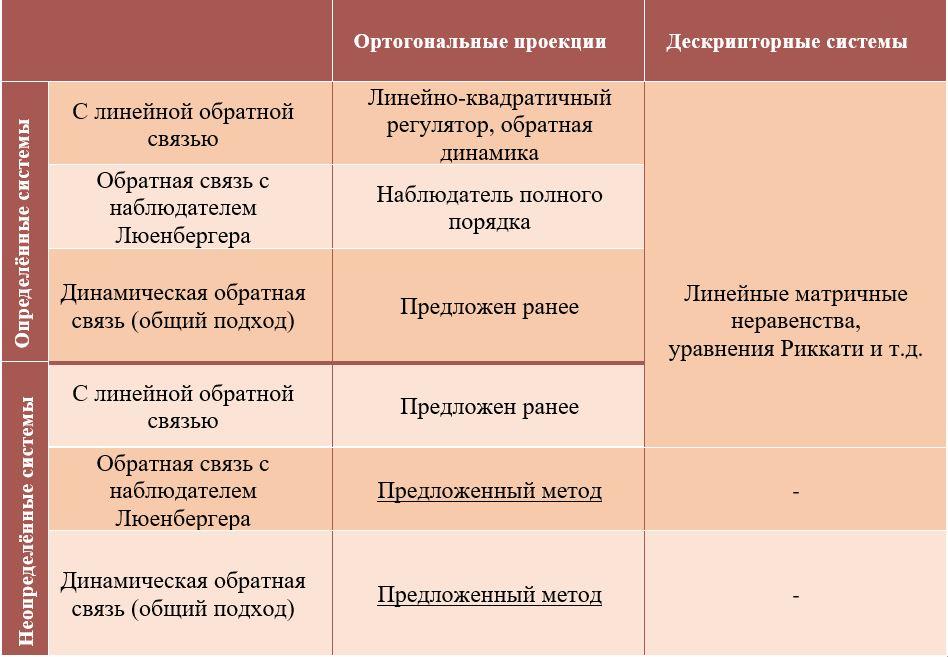
\includegraphics[scale=0.9]{images/table.JPG}
	}
	\caption{Диаграмма методов управления и оценки состояния для систем с явными ограничениями.}\label{fig:table}
\end{figure}

\section{Используемые математические инструменты}\label{sec:ch1/sec7}
В данной работе мы используем неравенство Юнга для решения проблемы билинейности, неопределённости в матрицах моделей также преобразовываются с помощью неравенства Юнга, дополнения Шура и S--процедуры.

Неравенство Юнга \cite{BOYED1994}, а также S--процедура \cite{Amato2011,LIEN2008} способствуют возникновению свободных скалярных параметров, которые могут внести нелинейность в задачу, особенно когда в ограничениях присутствует как переменная, так и ее инверсия. Решение этой проблемы было описано в \cite{KHELOUFI2016}, где один положительный скаляр и его инверсия были заменены двумя независимыми положительными скалярами. Другая проблема возникает, когда эти скалярные параметры вводят билинейность в задачу. Для этого случая, в \cite{KHELOUFI2013} был предложен метод решетчатого поиска, позволяющий превратить одну билинейную задачу в серию выпуклых задач с ограничениями в виде линейных матричных неравенств.

Дополнение Шура впервые было описано в \cite{Schur} для доказательства леммы Шура. В данной работе дополнение используется для преобразования суммы блочных матриц в одну блочную матрицу для линеаризации переменных в линейных матричных неравенствах.
\FloatBarrier
